\documentclass[addpoints]{exam}
\usepackage[utf8]{inputenc}
\usepackage[portuguese]{babel}
\usepackage[LGRgreek]{mathastext}
\usepackage{graphicx,graphics}
\usepackage{hyperref}
%\usepackage{framed}
\usepackage{multirow}
\usepackage{booktabs}

%%% INÍCIO DOS COMANDOS ACRESCENTADOS NO NETBOOK %%%%%%%%%%%%%%%%%%%
\newcommand*{\renameenviron}[1]{%
  \expandafter\let\csname exam-#1\expandafter\endcsname
      \csname #1\endcsname
  \expandafter\let\csname endexam-#1\expandafter\endcsname
      \csname end#1\endcsname
  \expandafter\let\csname #1\endcsname\relax
  \expandafter\let\csname end#1\endcsname\relax
}
\renameenviron{framed}
\renameenviron{shaded}
\renameenviron{leftbar}
%%% FIM DOS COMANDOS ACRESCENTADOS NO NETBOOK %%%%%%%%%%%%%%%%%%%
\usepackage{framed}

\footer{}{\thepage}{}

\renewcommand{\arraystretch}{1.3}
%\setlength{\tabcolsep}{pt}
 
\pointpoints{ponto}{pontos}
\bonuspointpoints{ponto extra}{pontos extra}
 
\totalformat{Pregunta \thequestion: \totalpoints pontos}
 
\chqword{Pregunta}
\chpgword{Página}
\chpword{Pontos}
\chbpword{Pontos extra}
\chsword{Pontos obtidos}
\chtword{Total}

\hqword{Questão}
\hpgword{Página}
\hpword{Pontos}
\hsword{Pontos obtidos}
\htword{Total}

 
\begin{document}
 
\large

\begin{center}
\Large
\textbf{Laboratório de Eletrônica Básica II – EE641}
\end{center}

\large
\vspace{2mm}

\noindent\textbf{Profs.:} Dr. Eduardo T. Costa\hfill \textbf{Turma 01/2022} \\
\textbf{PED:} Mathias Scroccaro Costa \hfill %\textbf{e-mail:} mathias.scroccaro@gmail.com

\normalsize
 
\vspace{5mm}
 

 
\noindent\makebox[0.72\textwidth]{Nome: \enspace\hrulefill}
\hfill
\makebox[0.2\textwidth]{RA: \enspace\hrulefill}

\vspace{5mm}

\noindent\makebox[0.72\textwidth]{Nome: \enspace\hrulefill}
\hfill
\makebox[0.2\textwidth]{RA: \enspace\hrulefill}

\vspace{5mm}

\noindent\makebox[0.72\textwidth]{Nome: \enspace\hrulefill}
\hfill
\makebox[0.2\textwidth]{RA: \enspace\hrulefill}



%\begin{center}
%\gradetable[h][questions]
%\end{center}

\vspace{2mm}


\begin{center}
\large
\textbf{REGULADORES LINEARES DE TENSÃO}
\normalsize
\end{center}

\begin{questions}

\section*{Fonte de alimentação +9 V e -9 V}

\question Monte o circuito regulador de tensão simétrico com os dispositivos LM7805 e LM7905, em \textbf{placa furada padrão}, como mostra o esquemático da Figura \ref{cir:1}. Utilize os valores de resistência R1 = 270 $\Omega$ e R2 = 220 $\Omega$. Consulte o \textit{datasheet} do dispositivo para o dimensionamento dos capacitores Cin e Cout. Antes de soldar os componentes na placa, complete a Tabela \ref{tab:0}. Não esqueça de soldar os conectores de alimentação e teste, pois serão \textit{fundamentais} em futuros experimentos. 
\begin{table}[h!]
\centering
\begin{tabular}{c|c|l|l|l|}
\cline{2-5}
\multicolumn{1}{l|}{} & \multicolumn{1}{l|}{Cin(medido)} & Cout(medido) & R1(medido) & R2 (medido) \\ \hline
\multicolumn{1}{|c|}{LM7805} &  &  &  &  \\ \hline
\multicolumn{1}{|c|}{LM7905} &  &  &  &  \\ \hline
\end{tabular}
\caption{Valores medidos dos componentes.}
\label{tab:0}
\end{table}


\begin{figure}[h!]
\begin{center}
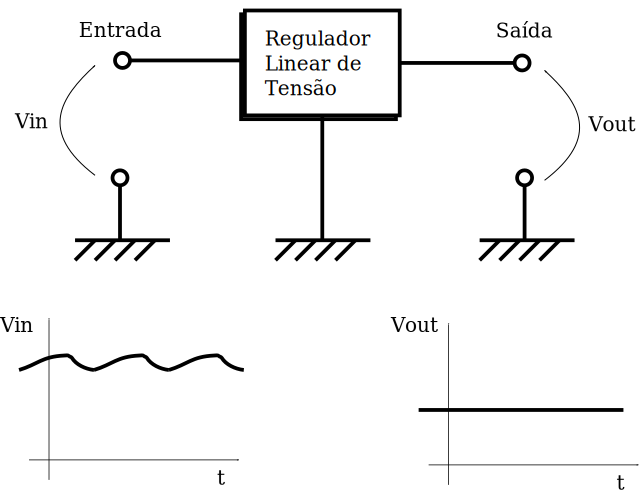
\includegraphics[width=0.8\textwidth]{imagens/reguladores.pdf}
\end{center}
\caption{Fonte de alimentação +9 V e -9 V.}
\label{cir:1}
\end{figure}

\begin{table}[h!]
\centering
\begin{tabular}{|c|c|c|c|c|c|c|}
\hline
\multicolumn{7}{|c|}{Regulador de tensão positiva} \\ \hline
\begin{tabular}[c]{@{}c@{}}Rload [$\Omega$]\\ (nominal)\end{tabular} & \begin{tabular}[c]{@{}c@{}}Rload [$\Omega$]\\ (medido)\end{tabular} & \begin{tabular}[c]{@{}c@{}}Vcc [V]\\ (nominal)\end{tabular} & \begin{tabular}[c]{@{}c@{}}Vcc [V]\\ (medido)\end{tabular} & \begin{tabular}[c]{@{}c@{}}nó +9 V [V]\\ (medido)\end{tabular} & \begin{tabular}[c]{@{}c@{}}Iload [mA]\\ (calculado)\end{tabular} & \begin{tabular}[c]{@{}c@{}}Pot. dissipada\\ LM7805 [mW]\\ (calculado)\end{tabular} \\ \hline
\multirow{3}{*}{100} & \multirow{3}{*}{} & 9 &  &  &  &  \\ \cline{3-7} 
 &  & 12 &  &  &  &  \\ \cline{3-7} 
 &  & 24 &  &  &  &  \\ \hline
\multirow{3}{*}{10 k} & \multirow{3}{*}{} & 9 &  &  &  &  \\ \cline{3-7} 
 &  & 12 &  &  &  &  \\ \cline{3-7} 
 &  & 24 &  &  &  &  \\ \hline
\end{tabular}
\caption{Regulador de tensão positiva.}
\label{tab:1}
\end{table}

\begin{table}[h!]
\centering
\begin{tabular}{|c|c|c|c|c|c|c|}
\hline
\multicolumn{7}{|c|}{Regulador de tensão negativa} \\ \hline
\begin{tabular}[c]{@{}c@{}}Rload [$\Omega$]\\ (nominal)\end{tabular} & \begin{tabular}[c]{@{}c@{}}Rload [$\Omega$]\\ (medido)\end{tabular} & \begin{tabular}[c]{@{}c@{}}Vss [V]\\ (nominal)\end{tabular} & \begin{tabular}[c]{@{}c@{}}Vss [V]\\ (medido)\end{tabular} & \begin{tabular}[c]{@{}c@{}}nó -9 V [V]\\ (medido)\end{tabular} & \begin{tabular}[c]{@{}c@{}}Iload [mA]\\ (calculado)\end{tabular} & \begin{tabular}[c]{@{}c@{}}Pot. dissipada\\ LM7905 [mW]\\ (calculado)\end{tabular} \\ \hline
\multirow{3}{*}{100} & \multirow{3}{*}{} & -9 &  &  &  &  \\ \cline{3-7} 
 &  & -12 &  &  &  &  \\ \cline{3-7} 
 &  & -24 &  &  &  &  \\ \hline
\multirow{3}{*}{10 k} & \multirow{3}{*}{} & -9 &  &  &  &  \\ \cline{3-7} 
 &  & -12 &  &  &  &  \\ \cline{3-7} 
 &  & -24 &  &  &  &  \\ \hline
\end{tabular}
\caption{Regulador de tensão negativa.}
\label{tab:2}
\end{table}

\pagebreak

\begin{parts}

\part Após a montagem, com auxílio de uma \textbf{protoboard}, aloque cargas resistivas: entre os nós +9 V e GND; - 9 e GND; conforme indicam as tabelas \ref{tab:1} e \ref{tab:2}, respectivamente. Complete os itens faltantes nas tabelas.  

\part (PÓS EXPERIMENTO) Explique como o circuito funciona. Comente sobre a potência dissipada sobre o regulador de tensão, conforme evidenciado nas Tabela \ref{tab:1} em \ref{tab:2}. 
\label{part:a}
\begin{framed}
\vspace{5cm}
\end{framed} 

\pagebreak

\part (PÓS EXPERIMENTO) Qual é a principal diferença entre os dispositivos da família 78XX e 79XX?
\begin{framed}
\vspace{5cm}
\end{framed}

\part (PÓS EXPERIMENTO) Explique como funciona o CI LM7805 internamente. (Desenhe diagramas de blocos, caso seja necessário)
\begin{framed}
\vspace{14cm}
\end{framed} 

\part (PÓS EXPERIMENTO) Qual a funcionalidade dos capacitores Cin e Cout?
\begin{framed}
\vspace{5cm}
\end{framed} 

\part (PÓS EXPERIMENTO) Se é possível fabricar capacitores em circuito integrado, por que tipicamente Cin e Cout são dispostos externamente no chip? Comente sobre a relação entre área no \textit{wafer} de semicondutor, custo de produção e valores de capacitância.
\begin{framed}
\vspace{6cm}
\end{framed}

\end{parts}


\end{questions}

\end{document}
